%%%%%%%%%%%%%%%%%%%%%%%%%%%%%%%%%%%%%%%%%%%%%%%%%%%%%%%%%%%%%%%%%%%%%%%%
% RevTeX 4.1 LaTeX
% Kevin C. Young
% Scalable & Secure Systems Research (08961)
% Thu Mar  5 15:29:19 PST 2015
%%%%%%%%%%%%%%%%%%%%%%%%%%%%%%%%%%%%%%%%%%%%%%%%%%%%%%%%%%%%%%%%%%%%%%%%

\documentclass[aps,nofootinbib,pra,notitlepage,twocolumn]{revtex4-1}
\usepackage{amsfonts,amsmath,amssymb,amsthm}
\usepackage{array,bm,color}
\usepackage{epsfig,graphicx,nomencl,revsymb4-1,upgreek,url}
\usepackage{hyperref}
\usepackage{algorithm}
\usepackage{algpseudocode}
\usepackage{graphicx}
\graphicspath{{./figures/}}
\hypersetup{colorlinks=true, pdfauthor=Kevin C. Young, pdftitle=Decorrelating Errors}
\newcommand{\tr}{{\rm Tr\thinspace}}
\newcommand{\bra}[1]{\ensuremath{\left\langle{#1}\right\vert}}
\newcommand{\ket}[1]{\ensuremath{\left\vert{#1}\right\rangle}}
\newcommand{\braket}[2]{\left\langle #1 | #2 \right\rangle}
\newcommand{\ketbra}[2]{\left| #1 \right\rangle\!\!\!\,\left\langle #2 \right|}
\newcommand{\abs}[1]{\left\vert #1 \right\vert}
\newcommand{\expect}[1]{\ensuremath{\left\langle{#1}\right\rangle}}
\newcommand{\timeorder}{\ensuremath{\underset{\leftarrow}{\mathcal{T}}}}
\newcommand{\ident}{{\mathbb1}}
\newcommand{\order}[1]{\mathcal{O}\left( #1 \right)}
\newcommand{\diag}[1]{\mathrm{diag}\{#1\}}
\newcommand{\trans}[1]{#1^\mathsf{T}}
\newcommand{\T}{\mathsf{T}}
\newcommand{\erf}[1]{Eq.~(\ref{#1})}
\newcommand{\needcite}{{\color{blue}\textsuperscript{[citation needed]}}}
\newcommand{\note}[1]{{\color{red}[#1]}}
\newcommand{\kcy}[1]{{\color{red}[#1]_{\rm{KCY}}}}
\newcommand{\amp}[1]{{\color{red}[#1]_{\rm{AMP}}}}

\newcommand{\actual}{\ensuremath{\tilde{\mathcal{G}}}}
\newcommand{\target}{\ensuremath{{\mathcal{G}}}}
\newcommand{\error}{\ensuremath{{\mathcal{E}}}}

%-------------Header begins here----------------------------------------
\begin{document}
\title{Advantages of mixed unitary operators for quantum information processing}

\author{Anthony Polloreno}
\email[Email: ]{anthony@rigetti.com}
\affiliation{Rigetti Computing, Berkeley, CA}

\author{Kevin C. Young}
\affiliation{Sandia National Laboratories, Livermore, CA}

\date{\today}

\begin{abstract}
...
\end{abstract}

\pacs{}

\maketitle


% ==============================================================================
% Section: Introduction
% ==============================================================================
\section{Introduction}
\label{sec:introduction}

The past decade has seen a dramatic increase in the performance and scale of quantum information processors (QIPs). Gate fidelities are now routinely in the 99\% to 99.99\% range, and dozens of individually-addressable qubits are becoming available on integrated devices. While these advances represent important steps forward on the path towards a computationally useful QIP, the quantum advantage milestone has yet to be definitively reached. The limiting factor, of course, is errors in the quantum gate operations.

The impact of an error in a quantum gate depends strongly on both the magnitude and nature of the errors. Systematic, or \emph{coherent}, errors can arise from poorly calibrated controls or imperfect gate compilations. These errors induce repeatable, undesired unitary errors on the state of a QIP. Errors of this type are correlated in time and add up coherently, so they are computationally expensive to model and it is difficult to place analytic bounds on circuit performance. Contrast this against random, or \emph{stochastic}, errors, which result from high-frequency noise in the controls or the environment. These errors can be modeled by defining a rate of various discrete errors in the system, such as a bit flip or phase flip. These errors are significantly easier to simulate on a classical computer, and their impact on quantum circuits is much easier to estimate.

Despite the relative ease of modeling stochastic errors, coherent errors are often much more likely to appear in QIPs. Drifting control parameters or environmental variables can easily have long correlation times that result in errors which is strongly coherent over the length of a quantum circuit. While these errors can often be reconstructed using various tomographic techniques, their impact is difficult to predict. The diamond distance can be used to estimate the failure probability of a quantum circuit, but the diamond distance can grow quadratically with repeated application of gate with coherent errors. For long circuits, this can add up extremely quickly. Recent work by Hastings and Campbell, however, has shown that coherent noise can be strongly suppressed by probabilistic sampling over various implementations of the target quantum gates. This averaging results in quantum processes with diamond distances that grow only linearly  quadratic in the over/under rotation angle of the component gates. \note{Clear this up.}

In this article we discuss various applications of mixed unitary controls, and show that the advantages of this approach can be made robust to drift in the target gates. In this article, we discuss an optimal control approach to the mixed unitary control design problem.  We apply our methods in simulation where we construct single- and two-qubit mixed unitary controls which are robust to drift and uncertainty in the control parameters. We further present an experimental implementation of single-qubit mixed unitary controls on a superconducting qubit testbed at Rigetti Quantum Computing. Using randomized benchmarking, we are able to show a marked improvement in error rates, as well as a reduced variance in circuit outcome probabilities, indicating a reduction in the coherence of the error.

% For instance, the repeated measurements that occur in quantum error correction are suspected to reduce the potential impact of coherent buildup of error. Modern devices, however, do not have sufficient numbers of qubits and their errors are above the threshold at which QEC becomes a viable option.


% ==============================================================================
% Section: Representing quantum gates
% ==============================================================================
\section{Representing quantum gates}
\label{sec:representing_quantum_gates}
The standard model for quantum gate operations is as linear maps on the state of some qubits. The state is usually represented as a density operator. It is often convenient, however, to represent the states instead as a generalized Bloch vector,
\begin{equation}
  \vec \rho = \tr(\rho \vec \sigma)
\end{equation}
Operations on this Bloch vector can then be represented as \emph{process matrices}, $\target$, and their action on a quantum state given by standard matrix multiplication
\begin{equation}
  \rho \rightarrow \target\rho = \error \actual \rho
\end{equation}
Here $\target_i$ is the target operation, $\actual$ is the actual gate as implemented, and $\error$ is the effective error channel. If the error channel is unitary, then the error is coherent. An advantage of this particular representation of quantum gates is that Pauli stochastic channels are diagonal, with each entry corresponding to the probability that the associated Pauli error occurs in a given application of the gate.

% ==============================================================================
% Section: Example Mixed Unitary Processes
% ==============================================================================
\section{Example Mixed Unitary Processes}
\label{sec:mixed_unitary_processes}
There are often many possibly ways of implementing a target quantum gate. Hastings and Campbell consider gates compiled using the Solovey-Kitaev algorithm, for which there are many choices of approximate quantum gate implementations. By implementing some number of these implementations at random, we are able to construct a quantum channel that has reduced coherent error. As a simple example, we have:

\begin{figure}
  \centering
  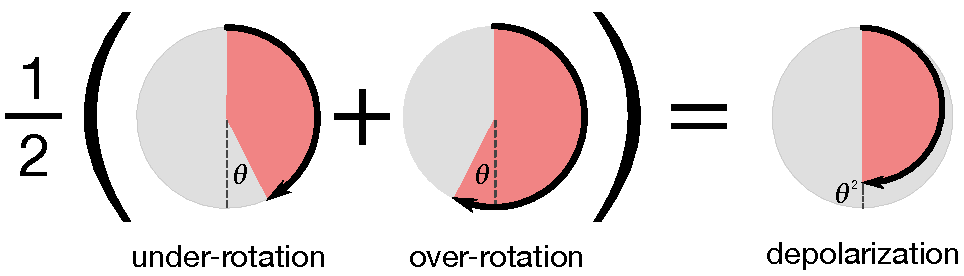
\includegraphics[width=\columnwidth]{simple_example.pdf}
  \caption{An example of a balanced control solution. Using optimal control, two implementations of a $Z_\pi$ gate are designed to have equal and opposite sensitivity to errors (if one implementation over-rotates by angle $\theta$, then the other \emph{under}-rotates by $\theta$). Each time the gate is used, one of these implementations is chosen at random. The resulting quantum channel is equivalent to a perfect implementation of the gate followed by dephasing of $\order{\theta^2}$.}
  \label{fig:simple_example}
\end{figure}

** This example is really useful and should be expanded. We should discuss the various optimization problems, a mixed unitary strategy, the fidelity of the resulting channel.


% ==============================================================================
% Section: Robustly Mixed Unitary Processes
% ==============================================================================
\section{Robustly Mixed Unitary Processes}
\label{sec:robustly_mixed}

\begin{figure}
  \centering
  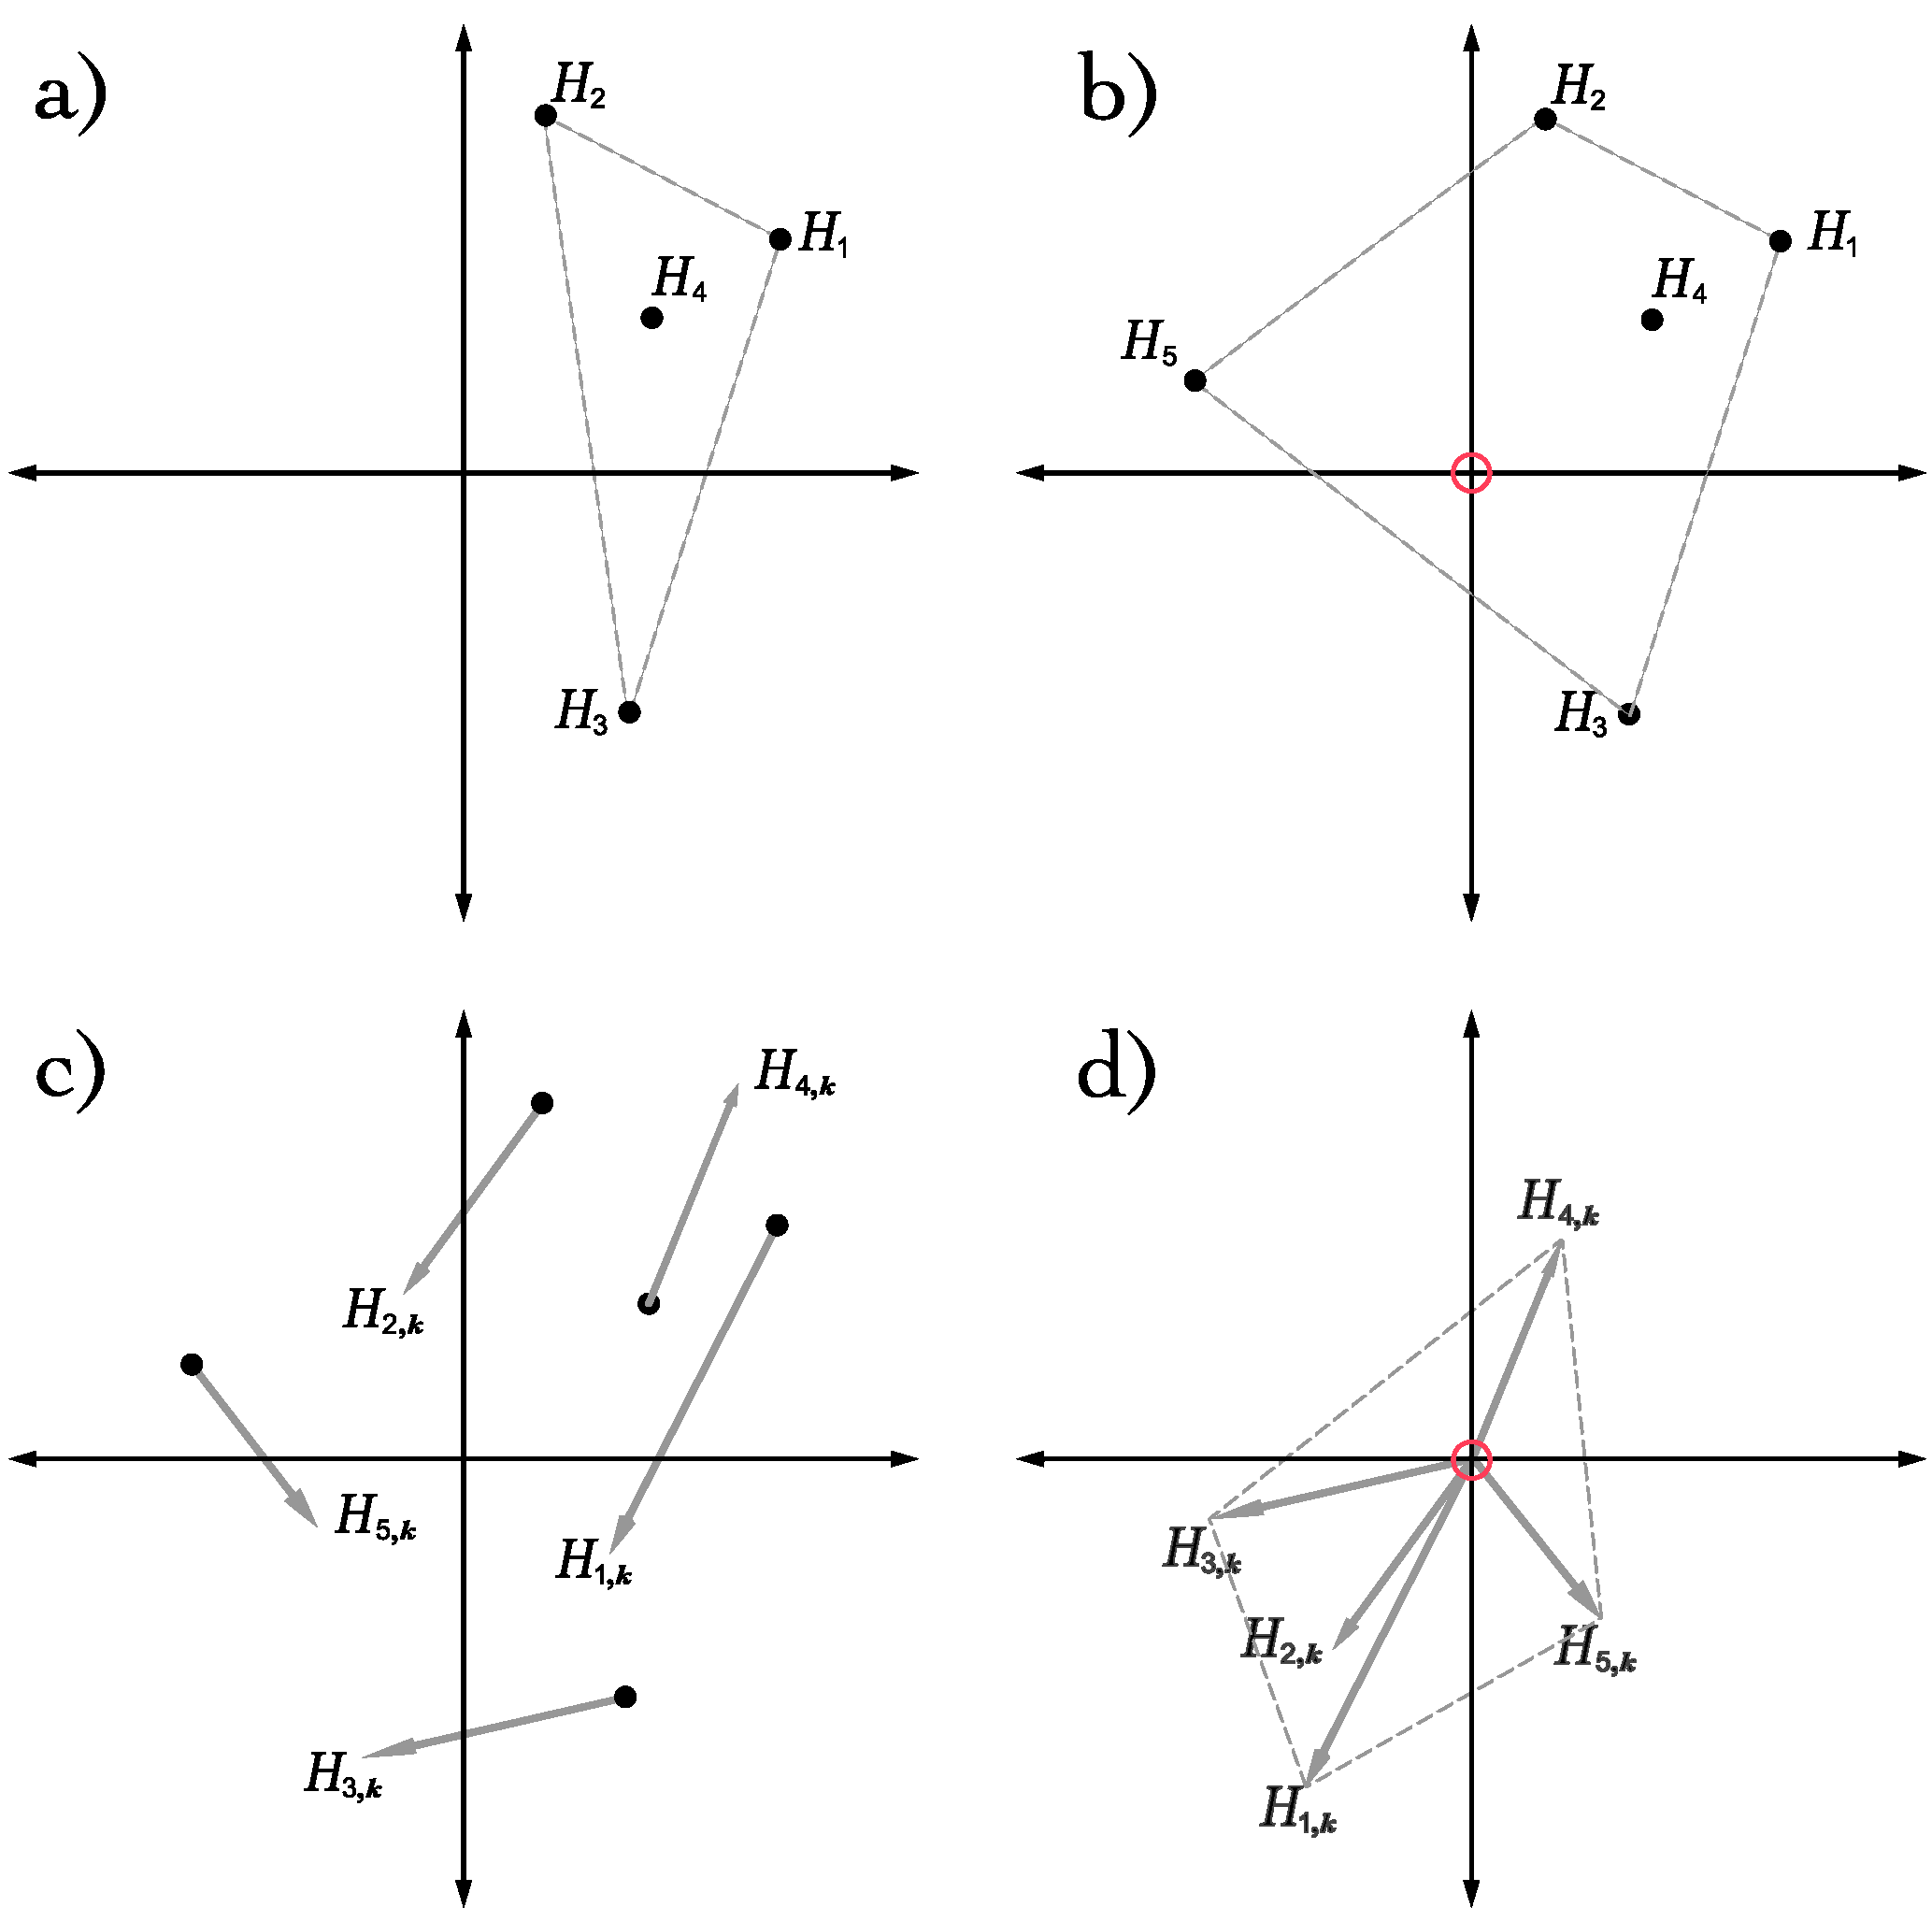
\includegraphics[width=\columnwidth]{vectorspace.pdf}
  \caption{A target unitary gate can be implemented a number of ways, each with a different effective Hamiltonian error. These error Hamiltonians lie in a vector space. a) Four effective Hamiltonians. The origin is not contained in their convex hull, so there are no balanced control solutions. b) The origin is contained in the covex hull after adding an additional control solution. Because there are more than $n+1$ implementations, there exist an infinite number of balanced control solutions. c) The error Hamiltonians shown with their derivative with respect to a control parameter. As this parameter drifts, a $0^{\rm th}$-order balanced control solution may drift, leading to a first-order error. d) The derivatives also lie in a vector space. If the origin lies in their convex hull, then it may be possible to construct a $1^{\rm{st}}$-order robust balanced control solution.}
  \label{fig:vectorspace}
\end{figure}


% ==============================================================================
% Section: Numerical Results
% ==============================================================================
\section{Numerical Results}
\label{sec:numerical_results}
In the following numerical results, we explore using the methods in Section \ref{sec:mixed_unitary_processes} to build MUPs. We consider the following model for a single tunable qubit: 
\begin{equation}\label{eq:1Qham}
  H(\delta, \epsilon, t) = \epsilon\sigma_z + (1 + \delta)(c_x(t)\sigma_x + c_y(t)\sigma_y)
\end{equation}
We use the GRAPE algorithm as discussed in \ref{sec:GRAPE} with N=25 steps and total evolution time of $\pi$ to generate 100 candidate controls. The performance function used to terminate the gradient descent was Equation (30) in \cite{Khaneja2005} -- the square of the Hilbert--Schmidt inner product between the generated unitary and the target unitary. The gradient, however, is the gaussian quadrature gradient described in \ref{sec:GRAPE}. In particular, using degree two (which should be accurate for polynomials up to degree 3) Gauss-Hermite quadrature we evaluated the gaussian weighted average gradient for standard deviation $\sigma=.001$, on both the qubit drive, and the qubit frequency. We assume that the errors on $\sigma_x$ and $\sigma_y$ are perfecly correlated, as in superconducting qubit systems that share a common RF drive.

Solving the optimization problem defined in  \ref{sec:robustly_mixed} with the MOSEK solver in \texttt{cvxpy} yields a 0MUP with nontrivial (nearly uniform 1\%) support on all the members of the control family. However, by imposing the sparsity constraint described in \ref{sec:robustly_mixed} the number of controls can be constrained to be just five. When generating a 1MUP we impose an $\ell1$ penalty so that the algorithm favors smaller error Hamiltonians.

In our two-qubit example we consider the following model for two tunable qubits coupled by a resonant exchange interaction, similar to that in \cite{McKay2016}:
\begin{equation} \label{eq:2Qham}
\begin{split}
H(\vec{\delta}, \vec{\epsilon}, t) = &\sum_{j=1}^2(\epsilon_j\sigma_z^j + (1 + \delta_j)(c_x^jx(t)\sigma_x^j + c_y^j(t)\sigma_y^j)) \\
&+ \frac{1}{10}(XX + YY)
\end{split}
\end{equation}

In this example it was infeasible to use GRAPE to return non-trivial solutions. Instead we manually selected piecewise constant echoing sequences with 500 steps and total evolution time of $\frac{5\pi}{2}$. In particular, we considered $RX(\pi)$, $RX(-\pi)$, $RY(\pi)$ and $RY(-\pi)$ pulses used to decouple detuning errors as taking only one time step, to avoid significant errors arising from non-commutativity. The specific collection of bang-bang sequences \cite{bang-bang} considered were all combinations of simultaneous $\pi$ pulses activated at multiples of $8$ steps from the first time step, and the same multiple of $8$ steps prior to the last time step. To give the control family a variety of RF errors, we added on uniformly distributed errors to each $\pi$ pulse, between $-.25$\% and $.25$\%. This resulted in 1024 controls, over which we performed the convex optimization described in \ref{sec:robustly_mixed}, with neither sparisty, nor $\ell1$ constraints.
% ==============================================================================
% Section: Experimental Results
% ==============================================================================
\section{Experimental Results}
\label{sec:experimental_results}
Here we present experimental results from implementing our routine on a fixed-frequency superconducting transmon qubit. In particular, we used qubit 8 on the Rigetti 19Q-Acorn chip, whose characterization can be found in \cite{1712.05771}. To implement a MUP on this qubit, four incorrectly calibrated Gaussian pulses were produced by scaling the pulseshape amplitude for a calibrated 10 sample 50ns $RX(\frac{\pi}{2})$ pulse by $106.4\%$,  $103.9\%$, $93.7\%$ and $91.2\%$.

Using the COBYLA minimizer in \texttt{scipy.optimize}\cite{scipy} to perform constrained minimization via Sequential Quadratic Programming\cite{wright1999numerical}, we minimized the off--diagonal elements of the resulting mixed process. \note{Explain why this an okay thing to do, or reference the section where we explain it.} To benchmark the quality of the new MUP, we then performed six randomized benchmarking experiments\cite{Magesan2011}: one for each over-- and under--calibrated pulse, one for the calibrated pulse, and one for the mixed process. We used $1000$ shots per experiment, $10$ sequences per sequence length, for sequence lengths of $2, 4, 8, 16, 32$ and $64$. In each case, our Clifford operations were decomposed into RX($\frac{\pi}{2})$) and RY($\frac{\pi}{2})$) pulses. In our implementation, these gates are implemented using the same pulse envelope definitions and control electronics, phase shifted by $\frac{\pi}{2}$ radians, and are therefore subject to identical miscalibration errors. The results are shown in Figure \ref{fig:rb} for sequence lengths $L=64$. The complete dataset can be found at  \cite{decorrelating_errors}.

Using \texttt{scipy.optimize.curve\_fit} to fit the randomized benchmarking data to Equation 6 in \cite{Magesan2011} with $B_0$ set to .5, and bounds between (0, 1), we find one-qubit gate fidelities of $99.3\%$ for the calibrated pulse, $98.9\%$ for Pulse1, $99.1\%$ for Pulse2, $98.9\%$ for Pulse3, $98.5\%$ for Pulse4, and $99.2\%$ for the MUP. In the cases of each miscalibrated pulse, the second moment of the RB number\cite{Proctor2017} for the sampled sequences extends significantly, which is in agreement with the results shown in \cite{Ball2016}. Specifically, for non-Markovian error models noise will manifest as gamma distributed points for each sequence length. On the other hand, Markovian noise, such as depolarizing noise, will result in Gaussian distributed fidelity estimates for each randomized benchmarking sequence length. We see that the coherently miscalibrated controls have long tails, consistent with gamma distributed random variables, while the calibrated and randomized implementations both have much shorter tails, consistent with Gaussian distributed random variables. 

\begin{figure}
  \centering
  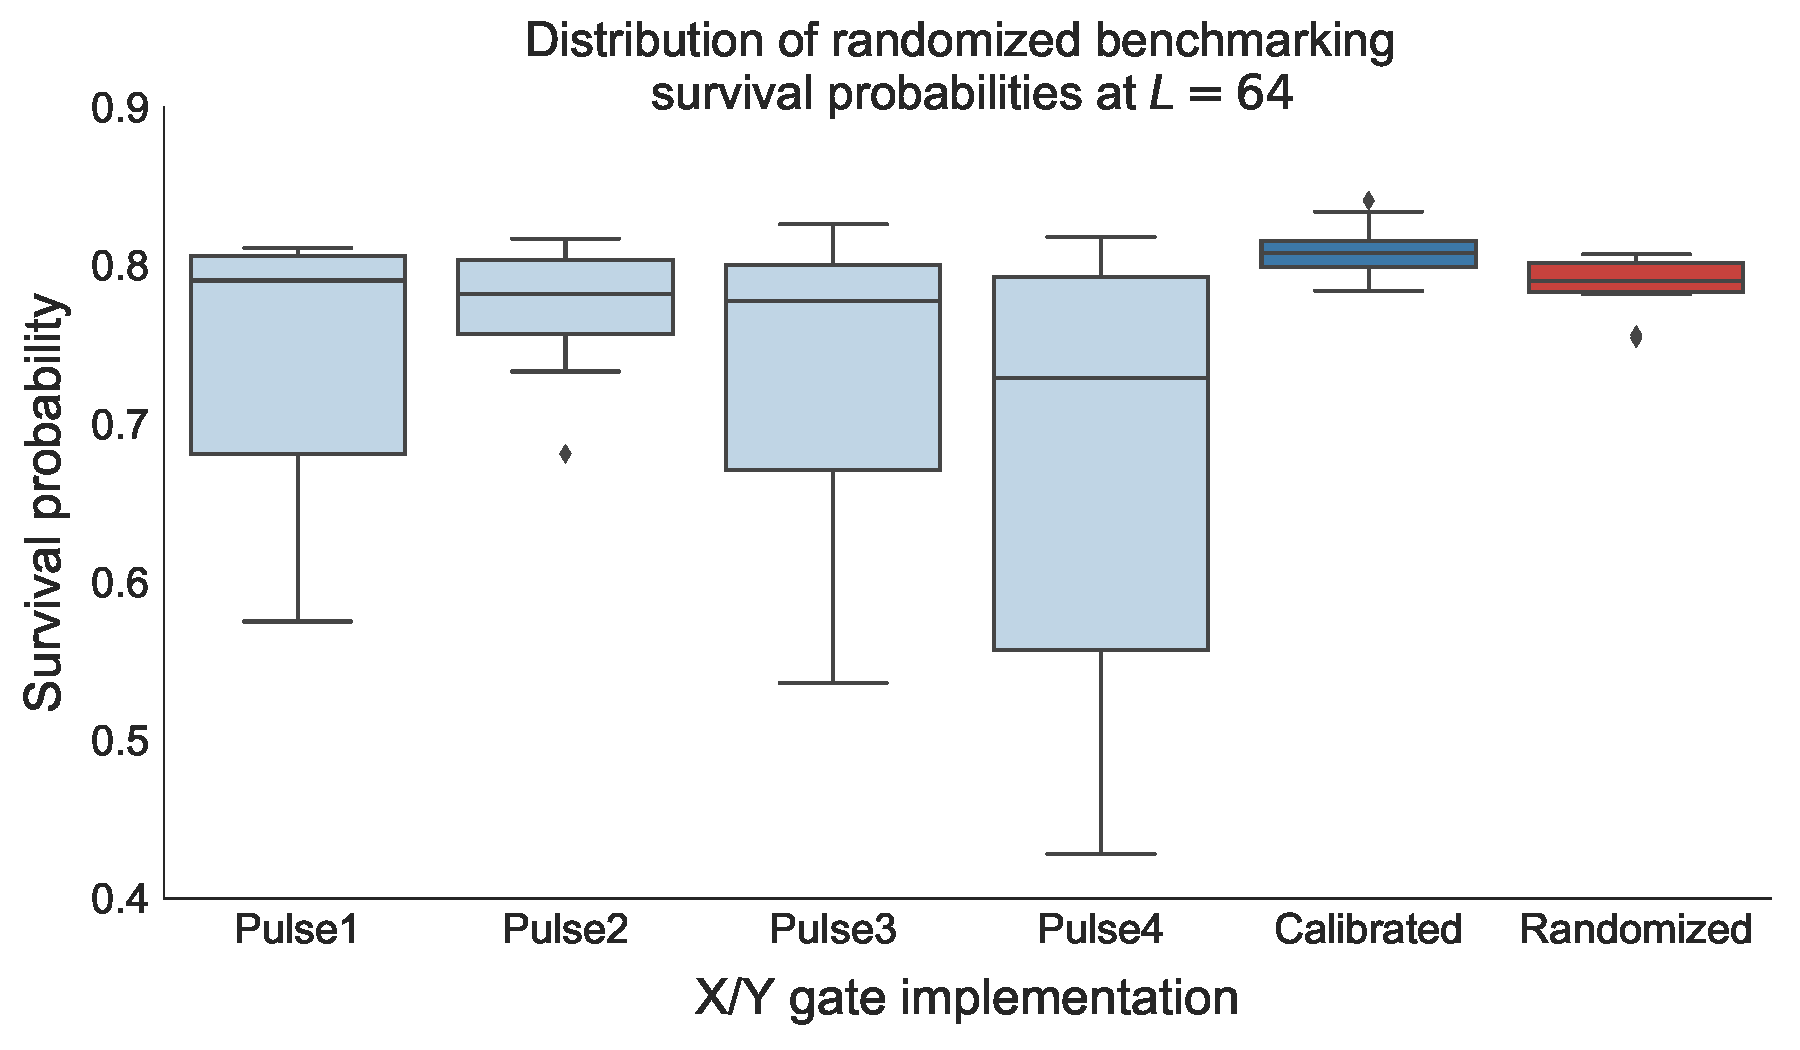
\includegraphics[width=\columnwidth]{rb_data.pdf}
  \caption{Randomized benchmarking experiments ran using different pulse definitions. The four plots on the left are from the incorrectly calibrated pulse, while the top right is the calibrated pulse, and the bottom right is the BCS.}
  \label{fig:rb}
\end{figure}




% ==============================================================================
% Section: Figures
% ==============================================================================
\section{Figures}
\label{sec:figures}

\begin{figure}
  \centering
  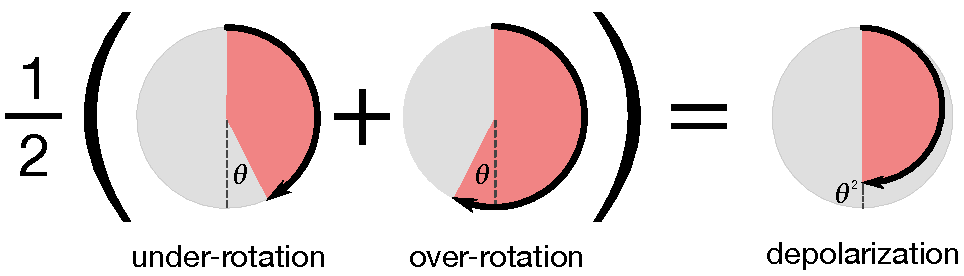
\includegraphics[width=\columnwidth]{simple_example.pdf}
  \caption{An example of a balanced control solution. Using optimal control, two implementations of a $Z_\pi$ gate are designed to have equal and opposite sensitivity to errors (if one implementation over-rotates by angle $\theta$, then the other \emph{under}-rotates by $\theta$). Each time the gate is used, one of these implementations is chosen at random. The resulting quantum channel is equivalent to a perfect implementation of the gate followed by dephasing of $\order{\theta^2}$.}
  \label{fig:simple_example}
\end{figure}

\begin{figure}
  \centering
  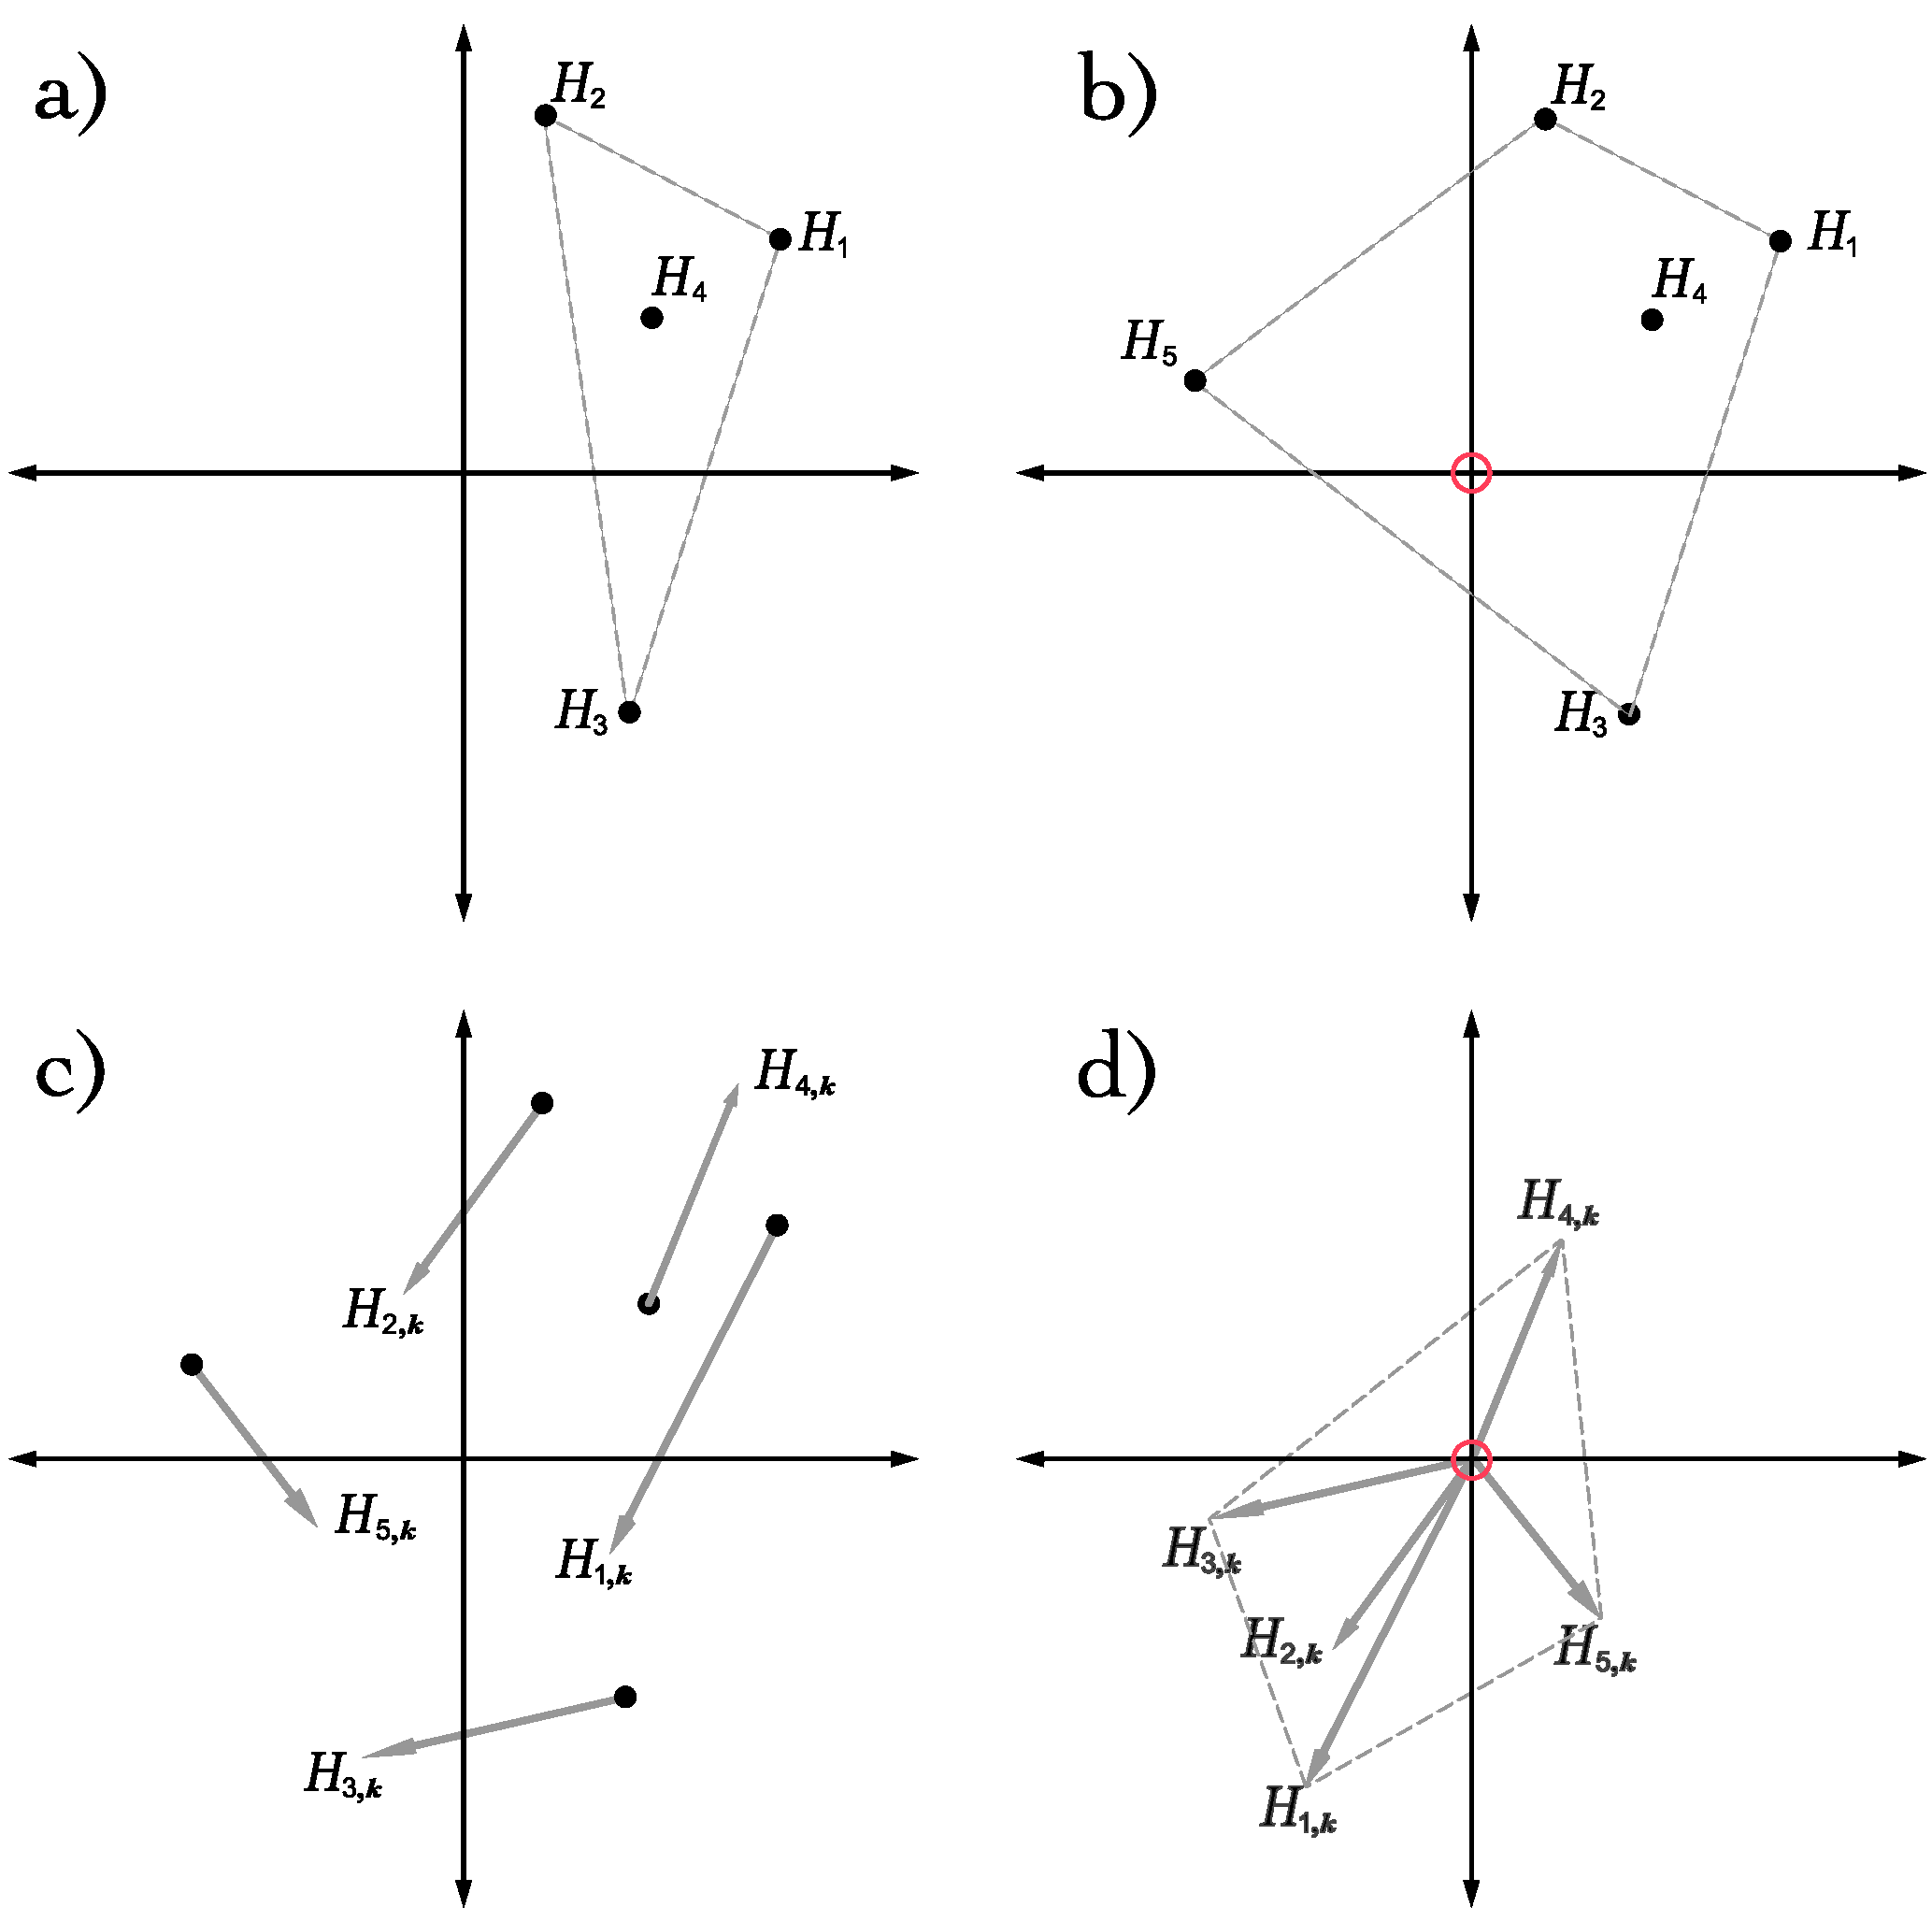
\includegraphics[width=\columnwidth]{vectorspace.pdf}
  \caption{A target unitary gate can be implemented a number of ways, each with a different effective Hamiltonian error. These error Hamiltonians lie in a vector space. a) Four effective Hamiltonians. The origin is not contained in their convex hull, so there are no balanced control solutions. b) The origin is contained in the covex hull after adding an additional control solution. Because there are more than $n+1$ implementations, there exist an infinite number of balanced control solutions. c) The error Hamiltonians shown with their derivative with respect to a control parameter. As this parameter drifts, a $0^{\rm th}$-order balanced control solution may drift, leading to a first-order error. d) The derivatives also lie in a vector space. If the origin lies in their convex hull, then it may be possible to construct a $1^{\rm{st}}$-order robust balanced control solution.}
  \label{fig:vectorspace}
\end{figure}

\begin{figure}\label{fig:num}
  \centering
  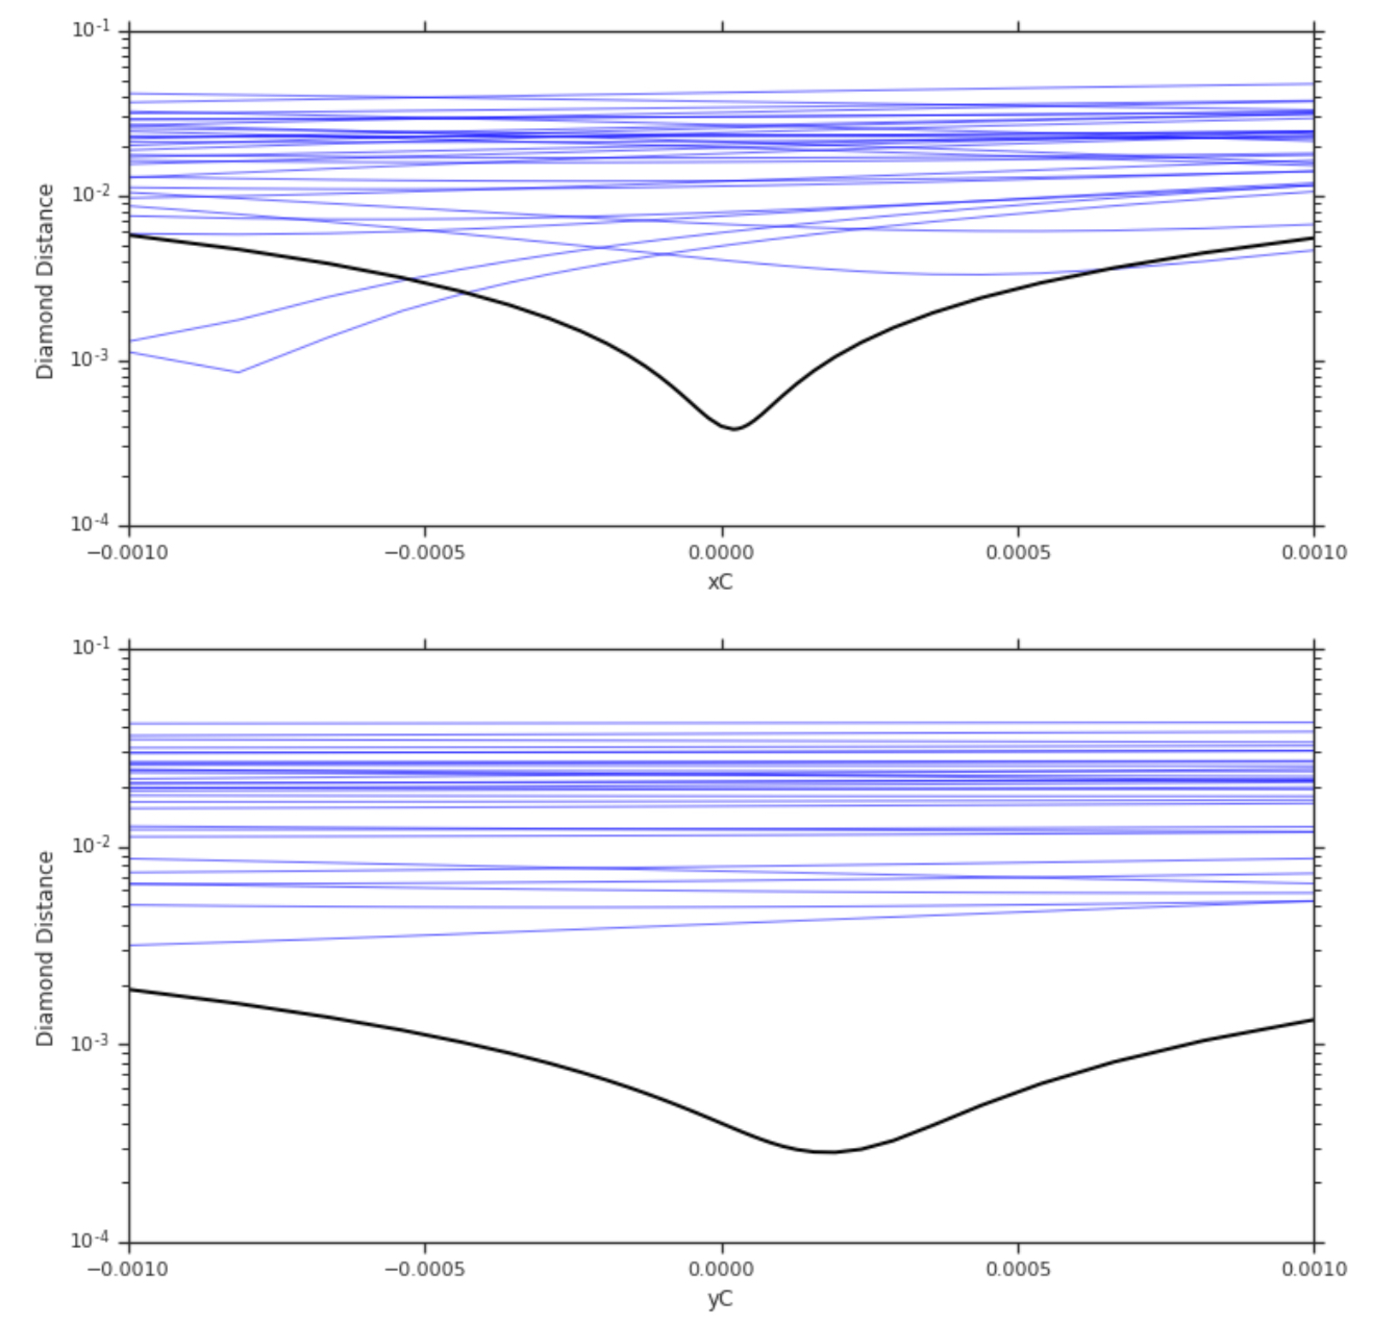
\includegraphics[width=\columnwidth]{placeholdernumerical.pdf}
  \caption{Placeholder image until we figure out what to plot. This currently shows that for one of the control the diamond norm decreased by over an order of magnitude. The labels need to be bigger.}
  \label{fig:rb}
\end{figure}


\begin{figure}
  \centering
  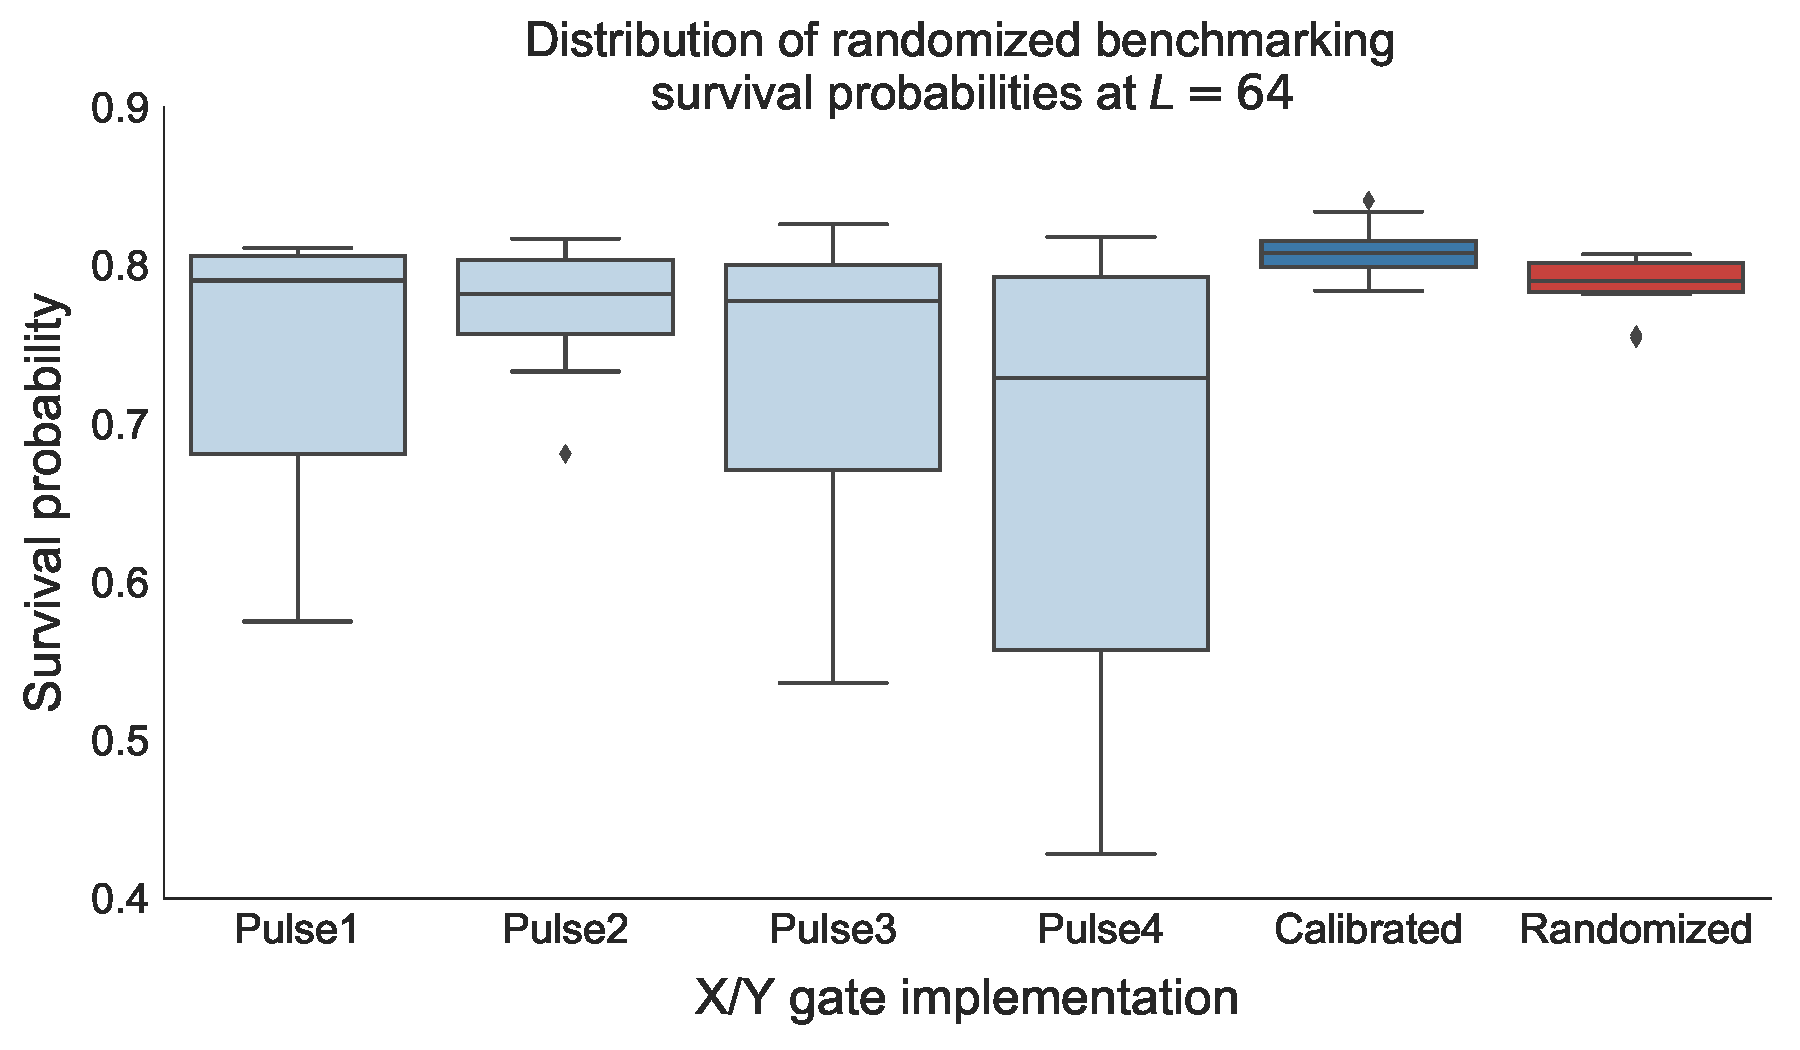
\includegraphics[width=\columnwidth]{rb_data.pdf}
  \caption{Randomized benchmarking experiments ran using different pulse definitions. The four plots on the left are from the incorrectly calibrated pulse, while the top right is the calibrated pulse, and the bottom right is the BCS.}
  \label{fig:rb}
\end{figure}

% ==============================================================================
% Section: Acknowledgements
% ==============================================================================
\section{Acknowledgements}
\label{sec:acknowledgements}
Sandia National Laboratories is a multimission laboratory managed and operated by National Technology and Engineering Solutions of Sandia, LLC, a wholly owned subsidiary of Honeywell International, Inc., for the U.S. Department of Energy's National Nuclear Security Administration under contract DE-NA0003525.
\bibliography{decorrelation.bib}
\end{document}
